% id: 149-299
% book: 개념원리 미적분Ⅰ · 17 속도와 가속도
% section: 필수·발전 예제
% figure: crop:fig-149-299.png
% answer: ⑴ $3\mkern3mu \mathrm{m/s}$ ⑵ $1.2\mkern3mu \mathrm{m/s}$
% answer_source: 답지
% variant_level: 0 (원본 전사)
% 이 파일은 build.mjs 가 items.json 에서 만든다. 고칠 때는 items.json 을 고친다.
\smash{\raisebox{1.5mm}{\dmkichul{개념원리 미적분Ⅰ 149쪽 299번 · 확인체크}}}
\noindent\begin{minipage}[t]{0.58\linewidth}\vspace{0pt}\raggedright 키가 $1.6\mkern3mu \mathrm{m}$인 민지가 $4\mkern3mu \mathrm{m}$ 높이의 가로등 바로 밑에서 출발하여 일직선으로 매초 $1.8\mkern3mu \mathrm{m}$의 일정한 속도로 걸어갈 때, 다음을 구하시오.\end{minipage}\hfill\begin{minipage}[t]{0.4\linewidth}\vspace{0pt}\centering \setlength{\dmfigw}{91.9pt}\ifdim\dmfigw>\linewidth\setlength{\dmfigw}{\linewidth}\fi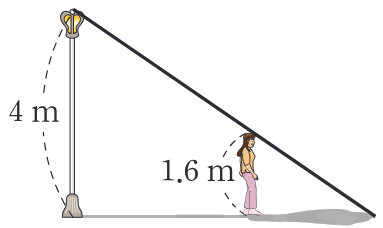
\includegraphics[width=\dmfigw]{figures/fig-149-299.png}\end{minipage}\par
\dmsubprob{1} 민지의 그림자의 머리끝이 움직이는 속도
\dmsubprob{2} 민지의 그림자의 길이의 변화율
